\documentclass[man]{apa6}
\usepackage{lmodern}
\usepackage{amssymb,amsmath}
\usepackage{ifxetex,ifluatex}
\usepackage{fixltx2e} % provides \textsubscript
\ifnum 0\ifxetex 1\fi\ifluatex 1\fi=0 % if pdftex
  \usepackage[T1]{fontenc}
  \usepackage[utf8]{inputenc}
\else % if luatex or xelatex
  \ifxetex
    \usepackage{mathspec}
  \else
    \usepackage{fontspec}
  \fi
  \defaultfontfeatures{Ligatures=TeX,Scale=MatchLowercase}
\fi
% use upquote if available, for straight quotes in verbatim environments
\IfFileExists{upquote.sty}{\usepackage{upquote}}{}
% use microtype if available
\IfFileExists{microtype.sty}{%
\usepackage{microtype}
\UseMicrotypeSet[protrusion]{basicmath} % disable protrusion for tt fonts
}{}
\usepackage{hyperref}
\hypersetup{unicode=true,
            pdftitle={The title},
            pdfauthor={First Author~\& Ernst-August Doelle},
            pdfkeywords={keywords},
            pdfborder={0 0 0},
            breaklinks=true}
\urlstyle{same}  % don't use monospace font for urls
\usepackage{graphicx,grffile}
\makeatletter
\def\maxwidth{\ifdim\Gin@nat@width>\linewidth\linewidth\else\Gin@nat@width\fi}
\def\maxheight{\ifdim\Gin@nat@height>\textheight\textheight\else\Gin@nat@height\fi}
\makeatother
% Scale images if necessary, so that they will not overflow the page
% margins by default, and it is still possible to overwrite the defaults
% using explicit options in \includegraphics[width, height, ...]{}
\setkeys{Gin}{width=\maxwidth,height=\maxheight,keepaspectratio}
\IfFileExists{parskip.sty}{%
\usepackage{parskip}
}{% else
\setlength{\parindent}{0pt}
\setlength{\parskip}{6pt plus 2pt minus 1pt}
}
\setlength{\emergencystretch}{3em}  % prevent overfull lines
\providecommand{\tightlist}{%
  \setlength{\itemsep}{0pt}\setlength{\parskip}{0pt}}
\setcounter{secnumdepth}{0}
% Redefines (sub)paragraphs to behave more like sections
\ifx\paragraph\undefined\else
\let\oldparagraph\paragraph
\renewcommand{\paragraph}[1]{\oldparagraph{#1}\mbox{}}
\fi
\ifx\subparagraph\undefined\else
\let\oldsubparagraph\subparagraph
\renewcommand{\subparagraph}[1]{\oldsubparagraph{#1}\mbox{}}
\fi

%%% Use protect on footnotes to avoid problems with footnotes in titles
\let\rmarkdownfootnote\footnote%
\def\footnote{\protect\rmarkdownfootnote}


  \title{The title}
    \author{First Author\textsuperscript{1}~\& Ernst-August
Doelle\textsuperscript{1,2}}
    \date{}
  
\shorttitle{Title}
\affiliation{
\vspace{0.5cm}
\textsuperscript{1} Wilhelm-Wundt-University\\\textsuperscript{2} Konstanz Business School}
\keywords{keywords\newline\indent Word count: X}
\usepackage{csquotes}
\usepackage{upgreek}
\captionsetup{font=singlespacing,justification=justified}

\usepackage{longtable}
\usepackage{lscape}
\usepackage{multirow}
\usepackage{tabularx}
\usepackage[flushleft]{threeparttable}
\usepackage{threeparttablex}

\newenvironment{lltable}{\begin{landscape}\begin{center}\begin{ThreePartTable}}{\end{ThreePartTable}\end{center}\end{landscape}}

\makeatletter
\newcommand\LastLTentrywidth{1em}
\newlength\longtablewidth
\setlength{\longtablewidth}{1in}
\newcommand{\getlongtablewidth}{\begingroup \ifcsname LT@\roman{LT@tables}\endcsname \global\longtablewidth=0pt \renewcommand{\LT@entry}[2]{\global\advance\longtablewidth by ##2\relax\gdef\LastLTentrywidth{##2}}\@nameuse{LT@\roman{LT@tables}} \fi \endgroup}


\DeclareDelayedFloatFlavor{ThreePartTable}{table}
\DeclareDelayedFloatFlavor{lltable}{table}
\DeclareDelayedFloatFlavor*{longtable}{table}
\makeatletter
\renewcommand{\efloat@iwrite}[1]{\immediate\expandafter\protected@write\csname efloat@post#1\endcsname{}}
\makeatother
\usepackage{lineno}

\linenumbers

\authornote{Add complete departmental affiliations for each
author here. Each new line herein must be indented, like this line.

Enter author note here.

Correspondence concerning this article should be addressed to First
Author, Postal address. E-mail:
\href{mailto:my@email.com}{\nolinkurl{my@email.com}}}

\abstract{
One or two sentences providing a \textbf{basic introduction} to the
field, comprehensible to a scientist in any discipline.

Two to three sentences of \textbf{more detailed background},
comprehensible to scientists in related disciplines.

One sentence clearly stating the \textbf{general problem} being
addressed by this particular study.

One sentence summarizing the main result (with the words ``\textbf{here
we show}'' or their equivalent).

Two or three sentences explaining what the \textbf{main result} reveals
in direct comparison to what was thought to be the case previously, or
how the main result adds to previous knowledge.

One or two sentences to put the results into a more \textbf{general
context}.

Two or three sentences to provide a \textbf{broader perspective},
readily comprehensible to a scientist in any discipline.


}

\begin{document}
\maketitle

\section{Introduction}\label{introduction}

\subsection{Community Labor United}\label{community-labor-united}

Community Labor United (CLU) is a non-profit organization, operating in
the Greater Boston Area, that works with other community-based
establishments and labor unions across Massachusetts to cultivate
strategic campaigns that protect and promote the interests of low and
middle-income working class families ({\textbf{???}}). Their overall
goal is to promote policies that advocate for accessible jobs,
healthcare, childcare, housing and environmental justice for working
class households ({\textbf{???}}). Through their Our Care That Works
coalition that launched publicly this year, Community Labor United aims
to bring together various local cooperative groups to confront the child
care crisis in Massachusetts. More specific to this research, CLU was
interested in examining the inconsistencies in childcare within the
Greater Boston Area, caused by the negligence of the Department of Early
Education and Care (EEC). This investigative exploration into childcare
provision gaps within the Greater Boston Area will allow Community Labor
United to communicate to the EEC the demand for the standardization of
childcare within Massachusetts.

\subsection{EEC Literature Review}\label{eec-literature-review}

The Department of Early Education and Care's mission is to maintain the
growth and development of all children, by providing quality childcare
programs and resources for families within their communities
({\textbf{???}}). However, the research lead by Community Labor United
and their affiliated organizations shows that the EEC has been unable to
effectively execute their commitment for low and middle-income working
class families.\\
We will be adding more limitations after we receive some literature from
Sarah about the EEC and childcare! (Sorry, friend)

\subsection{Research Question}\label{research-question}

As stated before, the general goal for this research was to examine the
inconsistencies in the EEC by highlighting childcare provision gaps in
the Greater Boston Area. More specifically, this project focused on
illustrating a disparity in operating hours and capacity for childcare
providers on the neighborhood level and census tract level. Because
Community Labor United is concentrated on understanding how the low and
middle-income households are impacted by the current childcare system,
our project focused on emphasizing the childcare demands needed for
working class families. Additionally, CLU was interested in
concentrating on early education provision care, which encompasses
childcare for children ages five and under. For hours, we looked at how
the non-typical work week is affected by the early education provision
that is currently supplied, since people with low and middle-incomes
work at times that operate outside the typical 9:00am - 5:00pm job. We
wanted to understand if there were a sufficient number of childcare
facilities that could offer early education provision outside Monday -
Friday, 7:30am - 6:00pm, for people in the Greater Boston Area.
Similarly for capacity, we wanted to highlight the lack of available
slots for early education provision for working households with children
age five and under. This is because working-class families typically
have all parents in the household in the workforce, so it is crucial
that the childcare capacity supply matches the demand.\\
Individually, the child provision gaps in hours and capacity shows how
the Department of Early Education and Care has neglected low and
middle-income families in specific ways. However, we also think it's
important to understand how the interaction between lack of available
childcare hours and lack of early education provision spots impact these
households overall. To best convey that interaction, we compiled our
visualizations and supporting information on an easily accessible
platform. This allows for the user to quickly navigate the various maps
for hours and capacity, and also share these findings with all
appropriate parties. It is our hope that Community Labor United will be
able to use the visualizations we've created to motivate the Department
of Early Education to make reforms to the current childcare system to be
more accommodating for all families in Massachusetts, regardless of
occupation or availability.

\section{Method}\label{method}

In order to quantify the gap in supply and demand for childcare in
Boston, we decided to focus on the capacity of the existing childcare
providers in comparison to the number of children who need childcare, as
well as the hours that providers are able to provide childcare in
comparison to the hours when childcare is most needed by those who work
outside standard hours. These areas were chosen because both for their
urgency in affecting access to and need for childcare, as well as for
the lack of existing research that exists on the gaps between the
childcare that exists and the childcare that is needed.

\subsection{Data}\label{data}

The data from our main analyses consisted of two data sources, one
addressing the supply side of the gaps in childcare, and the other
addressing the demand. The supply data source we used was given to us by
\emph{Community Labor United}, and it was a collection of providers from
the Department of Early Education and Care (EEC) in Massachusetts. The
initial dataset consisted of 8,318 observations, with each row
representing a childcare provider in Massachusetts. Since our project
focused specifically on the Boston area, we filtered the dataset to
contain only cities in Boston, which left us with 764 remaining
childcare providers. The cities included were Allston, Boston, South
Boston, Brighton, Charlestown, Dorchester, East Boston, Hyde Park,
Jamaica Plain, Mattapan, Roslindale, Roxbury, and West Roxbury. Cities
with the highest concentration of providers included central Boston
(100), Dorchester (203) and Roxbury (70).

There is no existing dataset that tells us about childcare demand
specifically, so to answer this question we used census data,
specifically the \emph{American Community Survey} (ACS), and filtered
for certain variables of interest. The following methodology will
discuss specific variables in detail, but data was derived from the 2016
American Community Survey and was filtered for Suffolk County,
Massachusetts.

We wanted to convey the gap in childcare by a geography that would be
big enough to generalize findings, but small enough that we could be
specific and not overlook any areas that might have findings of
interest. Through consultation with CLU, we decided on convey our
results by the neighborhood level. To do this, we accessed Boston
neighborhood shapefile data ({\textbf{???}}) and assigned each EEC
childcare provider to a certain neighborhood. Since the census data of
interest was only accessible by tract, we developed a file that matched
each census tract to a neighborhood, and included both tract geometry
and neighborhood geometry to allow for easy mapping. More about this
process is discussed in the challenges section.

\section{Capacity}\label{capacity}

\subsection{Supply}\label{supply}

To get a sense of the slots available for early education provision, we
took the EEC dataset and filtered only for providers that provide early
education childcare. We first used R and Python to clean the variables.
We then used the tidyverse package to group the providers by census
tract, and calculated the total number of slots for early education
childcare in each tract. Since we were interested in looking at
differences on both the tract level and the neighborhood level, we
repeated this process for neighborhood so that we also had the total
number of slots for early education childcare in each neighborhood. We
merged these datasets with the respective geometry for each geography,
to allow us to map the results.

\subsection{Demand}\label{demand}

Demand for capacity of childcare was assessed through the use of the
2016 ACS. The tigris and tidycensus packages were used in congruence
with an API key to access census data in R. We chose the ACS as opposed
to other forms of census data because it was the only survey that was
easily compatible with R that also had all data available for all
variables of interest on the tract level for Suffolk County.

To quantify the number of children that need childcare, we used the ACS
variable \enquote{B23008}, which gives estimates per tract of the total
number of children under 6 years old, as well as the number of children
under 6 in two-parent households with both parents in the labor force,
as well as single parent households (either mother or a father) with the
parent in the labor force. We then added up these three variables, with
the assumption that anybody with all parents in the labor force would
need childcare. To get a percentage of children under 6 with all parents
in the labor force, we divided this number by the total number of
children under 6. All calculations were per tract.

\subsection{Maps}\label{maps}

Three maps were made as a final product for visualizing the gap in
capacity. Two of these maps (Figure 1 and Figure 2) looked at supply and
demand at the tract level, mapping the raw number of children under 6
with all parents in the workforce as well as the raw number of slots
available for early ed care per tract, to be compared. The third map
(Figure 3) quantified the difference in supply and demand by
neighborhood, as a ratio of children under 6 with parents in the
workforce to available childcare slots. Since it is unrealistic that one
would restrict their childcare search to within their census tract, a
rather small boundary, we wanted to give a more realistic range of how
far a childcare search might go, hence the rationale for grouping by
neighborhood.

\subsubsection{Hours}\label{hours}

\subsection{Supply}\label{supply-1}

Our main focus with the question of hours was to get a sense of the
providers who provided childcare outside of the typical standard
workday, which we defined as anytime outside of 7:30am-6pm on weekdays.
We did not include weekday care since there were only a few providers
that provided any weekend care at all. Therefore to get our dataset for
supply, we created a variable based on the information about hours in
the EEC dataset to flag any provider that provided care during
nonstandard hours, and summarized the number of slots they had for those
hours.

\subsection{Demand}\label{demand-1}

One large problem with census data is that in any workday related
variables, it assumes workers work 5 days a week, with the same number
of hours every day. This definition contradicts the purpose of our
study, which is to investigate those who work nonstandard hours.
Therefore, the only census variable that made sense to use when
investigating hours was the time leaving work. Using previous ACS
methodology given to us by CLU, we split the nonstandard times leaving
for work into three categories: early mornings if they leave for work
anytime between 12am-6:29am, evenings if they leave for work anytime
between 11am-3:59pm, late evening/overnight if they leave for work
anytime between 4pm-11:59pm. We took the ACS variables corresponding to
these responses in variable B08302, and divided the number of people in
each category by the total number of people in the workforce to get a
percentage of people in each category. We also summarized the number of
people in the three nonstandard time chunks to get a total percentage of
people leaving during any nonstandard hour.

\subsection{Maps}\label{maps-1}

Five maps were made to visualize the gap in supply and demand for hours.
Three of the maps were choropleth maps by tract visualizing the
percentage of people who left at each of the nonstandard times: early,
evening, and late evening/overnight (See Figure 1 for an example of this
map). Another similar map was made by tract using the aggregate
percentage of all people leaving during any of these nonstandard hours.
Finally, to visualize supply, a map was made of the number of slots
available for nonstandard hours of childcare by provider by tract.

\section{Results and Dsicussion}\label{results-and-dsicussion}

This section summarizes the data utilized and how the maps we create
illustrate the gap between demand and supply of childcare services for
children under 6 in the Boston area. We start by presenting the summary
statistics of the data sets, analyzing each individual map, and then
proceed to analyze the relationship among them.

\subsection{Summary Statistics}\label{summary-statistics}

Table 1 in the appendix presents the summary statistics on the
distribution of the capacities of all providers and capacities available
in neighborhoods and tracts. The mean capacity of providers is 24.7, of
all neighborhoods in Boston is 1469, and of tracts in Boston is 169.2.

Table 2 in the appendix presents the summary statistics on the
distribution of the capacities of all providers that operate outside
7:30am-6:00pm during weekdays and the capacities of them in
neighborhoods and tracts.

\subsection{Graphs for Capacity}\label{graphs-for-capacity}

In this section we conduct graphical analysis on the two variables we
are interested in: capacity and hours.

Figure 1 shows the number of children under 6 whose parents are in the
labor force (i.e., actively looking for jobs) on the level of
neighborhoods. We are especially in them since they are target consumers
of childcare services for early ed. Being in the labor force means that
the parents might to too busy to pay enough attention and provide enough
cares to their children, thus requiring the aids from childcare
providers. According to the map, tracts that have the largest number of
children under 6 who would need childcare services are mainly located in
the east and west parts of Boston (i.e., upper and lower regions on the
map), including East Boston, West Roxbury, Hyde Park, and Dorchester.

Figures 2 shows the number of childcare slots available for children
under 6 on the level of tracts. The two tracts that contain more slots
than others are located in Dorchester and Downtown, but compared to
Figure 2, the slots are apparently more evenly distributed across
tracts. It is worth paying attention to that providers in the regions
where there is a large number of children under 6, including the east
and west parts of Boston, do not provide enough number of slots to feed
the need of families in these areas. The difference between supply and
demand explains the high desert ratio in these regions as shown in
Figure 3.

We first visualize the gap between supply and demand for childcare
services for early education through the capacity variables. Figure 1
shows the ratio of children under age 5 to the cumulative child care
capacity in the neighborhoods of Boston. The darker the red color, the
more children are competing to obtain a licensed child care slot, and
therefore the harder it is for a child to obtain the childcare service
he/she needs. According to the graph, East Boston, Charlestown, South
Boston, Dorchester, Mattapan, Roslindale, Hyde Park, and West Roxbury
could be classified as child care deserts. To solve this issue, more
childcare providers should be established in those neighborhoods and
current providers should expand their capacities. To get a closer look
at the capacity, the two figures below show the demand and supply of
capacities by tracts.

\subsection{Graphs for Hours}\label{graphs-for-hours}

In this section, we look into the working hours of families and the
operating hours of providers to examine whether there is a mismatch.

Figure 4 shows the percentage of parents in tracts who depart for jobs
early in the morning. On average, people who live in the East Boston and
West Boston areas (north and south areas on the map) leave earlier for
works than people who live in other regions. These are also the regions
where there are relatively larger number of children under 6 in need of
childcare services. The tracts where the largest percentages of people
leave for jobs early are located at are waterfront areas of South Boston
and Dorchester.

Figure 5 shows the percentage of parents in tracts who leave for home in
the late evening. On average, people who live in the East Boston, West
Boston areas (north and south areas on the map), and waterfront tracts
Brighton and Allston leave from workplaces for home later than people
who live in other regions. The tracts where the largest percentages of
people leave for home later than usual are located at Roxbury and the
waterfront areas of Jamaica Plain.

Figure 6 shows the percentage of parents in tracts who depart for home
from the workplace overnight. On average, people who live in South
Boston and West Boston areas (north and south areas on the map) leave
later for home than people who live in other regions. These are also the
regions where larger percentage of people leave early and where there
are relatively larger number of children under 6 in need of childcare
services. The tracts where the largest percentages of people leave for
jobs early are located at are waterfront areas of South Boston and
Dorchester.

Figure 7 shows the number of slots available for early by providers that
open before 7:30am and close after 6pm during weekdays. It indicates
that there is a significant lack of capacities in regions where families
have a difficult commute time. In general, people from working families
living in East Boston, West Boston, South Boston, and the waterfront
areas of Allston, Brighton, and Jamaica Plain are most in need of off
hour childcare services. However, we could see that there are only a few
slots offered by childcare providers that operate off hour available for
children in West Boston and South Boston, and none for children in South
Boston and the waterfront areas of Allston, Brighton, and Jamaica Plain.
Accordingly, more off hour slots should be provided in these regions.

\section{Challenges and Limitations}\label{challenges-and-limitations}

\subsection{Challenges}\label{challenges}

There are two main challenges that we deal with for this project. First
is data cleaning for the EEC dataset. The EEC dataset has a messy data
format and a lot of columns that contain information on several
different variables. To extract information that we need to create the
capacity and hours variables, we utilize various functions and packages
from R and Python to clean, merge, and spread variables from the
original dataset, such as minimum age, rates, open and close time of
providers.

Second is the geographical classification. One of the narratives of this
project is to look at the supply and demand by the tract and
neighborhood levels, the information of which are not provided in the
original datasets we are given. We deal with this issue by geocoding the
providers' locations, deciding which polygon each provider falls within
using the over function from the rgeos package.

\subsection{Limitations}\label{limitations}

First some of the variables from census datasets are based on
assumptions different from real life situations. Specifically, people's
departure time for work is created based on the assumption that people
work for the same amount of hours everyday while the parents we are most
interested in are those that have irregular working hours.

Second, our general lack of ability to match census data variables with
variables EEC provide to compare different variables for the same
construct. Although we successfully create the desert ratio by using the
capacity and children population from the EEC and census datasets, there
are many other variables the project could look into, such as income
level of citizens vs.~subsidy of providers.

Third, there is a lack of data in the EEC dataset about important
variables, such as the capacity of each providers by age groups and
subsidy amount in dollars. The absence of these variables prevents us
from looking more deeply into the supply for childcare services. There
are many variables that we clean but do not look into due to the limited
amount of time we have, such as subsidy, availability of drop-in and
emergency services.

\section{Discussion and Conclusion}\label{discussion-and-conclusion}

To examine the inconsistencies in the EEC by highlighting childcare
provision gaps in the Greater Boston Area, we utilize EEC datasets and
census datasets to create maps that illustrate a disparity in operating
hours and capacity for childcare providers on the neighborhood level and
census tract level. In a word, East Boston and West Boston
neighborhoods, including Allston, Boston, South Boston, Brighton,
Charlestown, Dorchester, East Boston, Hyde Park, Jamaica Plain,
Mattapan, Roslindale, Roxbury, and West Roxbury, are the regions where
the gaps apparently exist. According to the visualizations of the
\enquote{capacity} variable, providers in East Boston and West Boston,
where there is a large number of children under 6, do not offer enough
number of slots to feed the need of families in these areas. Similarly,
the maps on the \enquote{hours} variable indicate that there is a lack
of childcare off hour services for working families living in East
Boston, West Boston, South Boston, and the waterfront areas of Allston,
Brighton, and Jamaica Plain are most in need of off hour childcare
services. According to the median income level map of Boston, most of
these neighborhoods are also regions where income levels are lower than
the average income level of the Boston area ({\textbf{???}}). The
limited financial capability of citizens of these areas might force them
to work during irregular hours and to send their children to the
childcare providers. On the other hand, the providers in these regions
could not provide enough slots for children under 6 as they could not
earn as much money from these low-income families as they could from
families in the central areas. To resolve the gap, the policy
intervention and support from EEC could be urgent.\\
In a word, our graphical analysis successfully illustrates the existence
of the gap between supply and demand for early ed childcare services in
the Boston area. For researchers who are interested in digging more
deeply into this topic in the future, we suggest several directions they
could explore into. First, people could match more variables on the
demand for childcare services with variables on the supply for childcare
services to illustrate the existence of gaps. Second, people could try
to obtain a more comprehensive dataset from EEC to have a closer look at
the supply of childcare services for different age groups. Third, people
could conduct a childcare survey by themselves to have first-hand
information directly from the providers and families in need of
childcare services in Boston. Fourth, people could encharge the studied
area to the whole mass

\section{Appendix}\label{appendix}

\begin{figure}
\centering
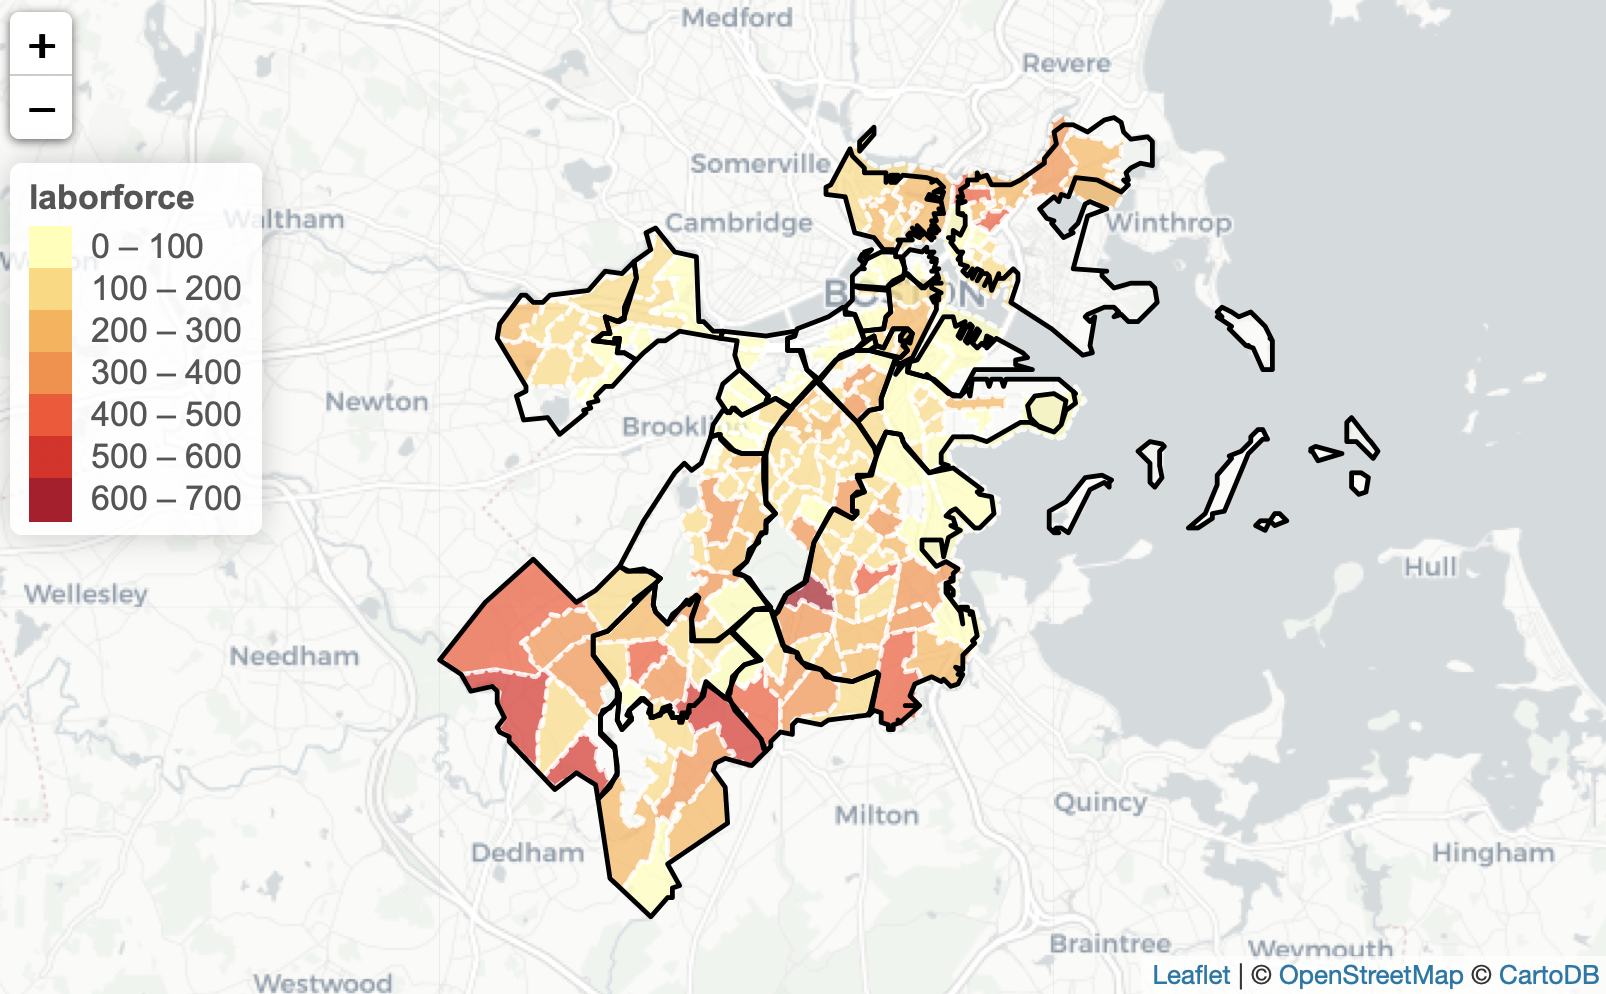
\includegraphics[width=5.20833in]{fig1.png}
\caption{Demand: Number of Children Under 6 with Parents in the Labor
Force}
\end{figure}

\begin{figure}
\centering
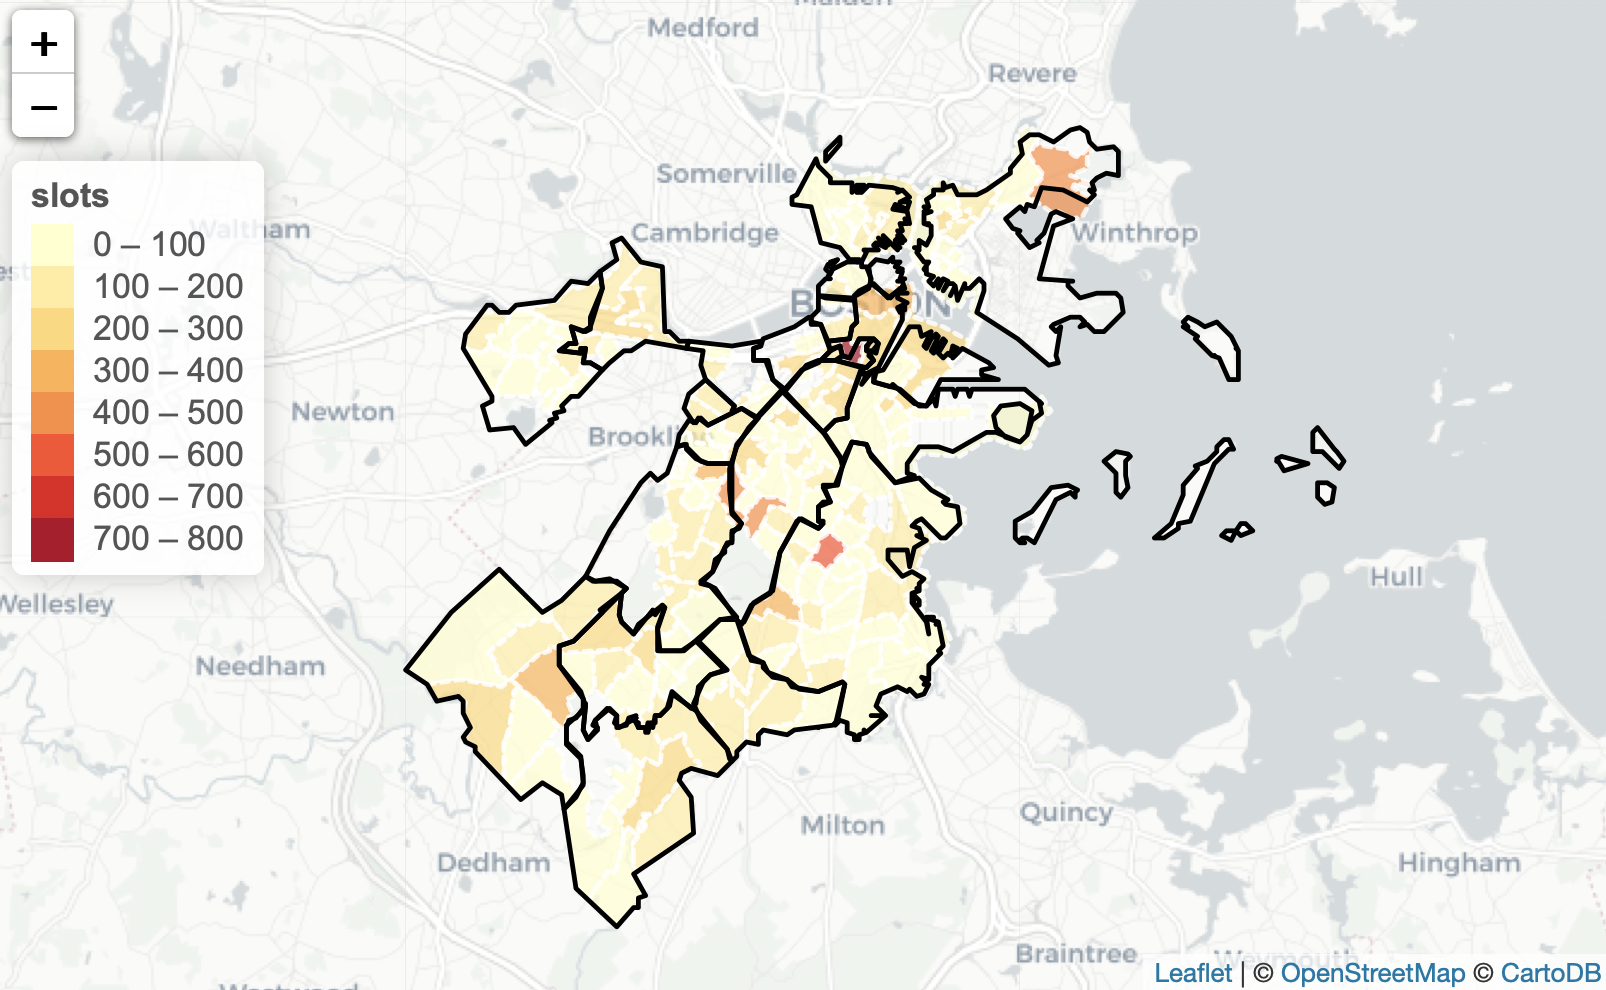
\includegraphics[width=5.20833in]{Fig 2, slots.png}
\caption{Number of slots available for early ed by tracts}
\end{figure}

\begin{figure}
\centering
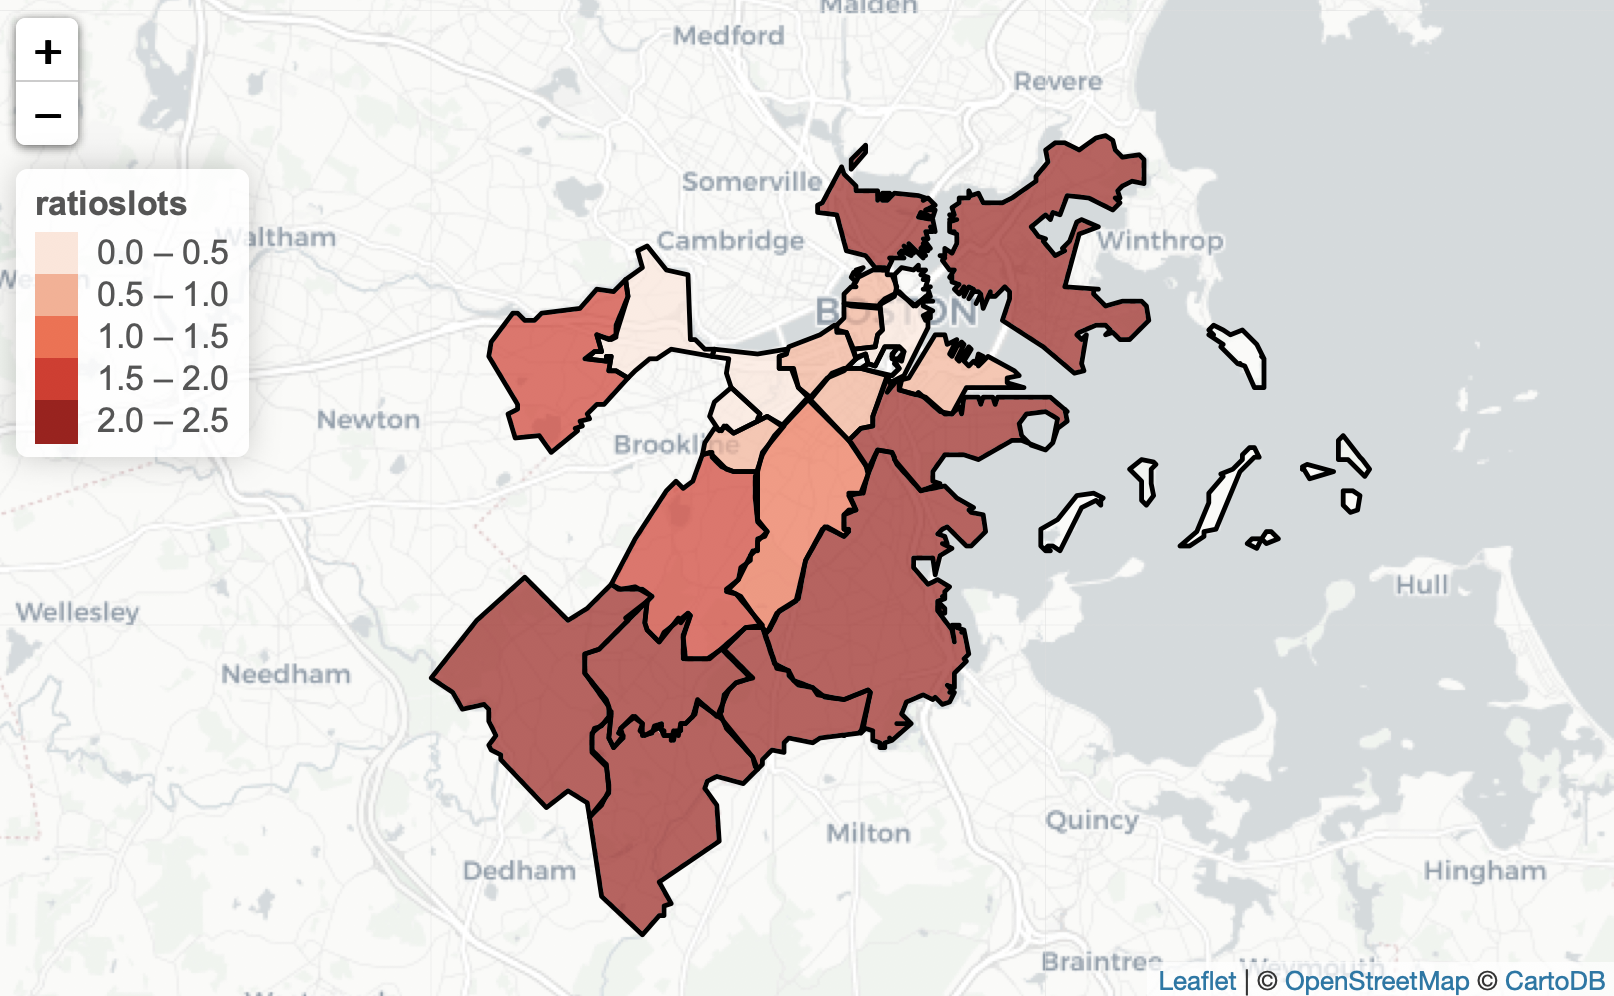
\includegraphics[width=5.20833in]{Fig 3, ratioslots.png}
\caption{Gap between supply and demand of capacities}
\end{figure}

\begin{figure}
\centering
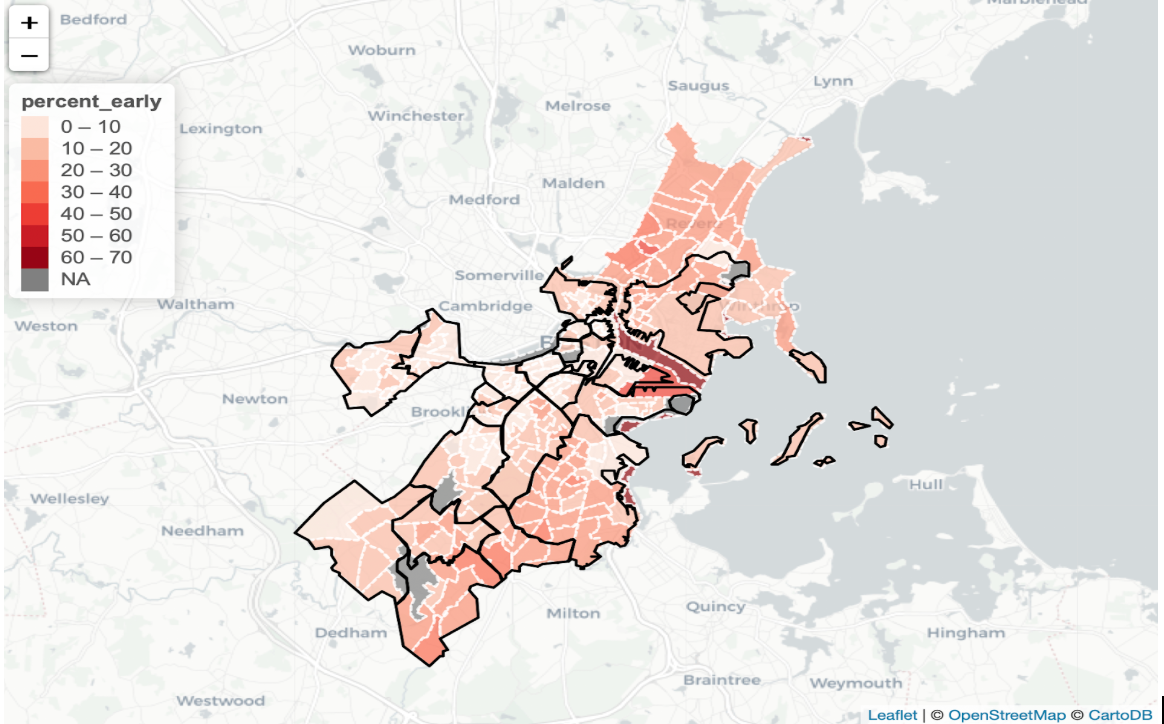
\includegraphics[width=5.20833in]{fig4.png}
\caption{Demand: Percentage maps by tracts on people departure time for
work in the morning}
\end{figure}

\begin{figure}
\centering
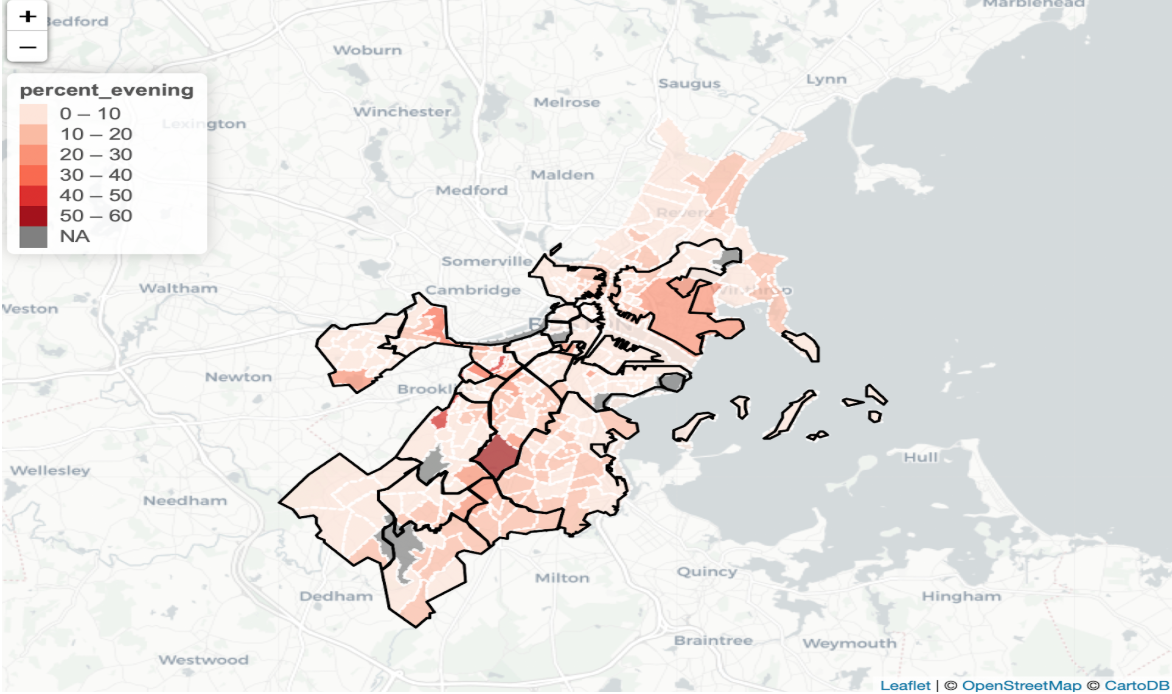
\includegraphics{fig5.png}
\caption{Demand: Percentage maps by tracts on people departure time for
home in the evening}
\end{figure}

\begin{figure}
\centering
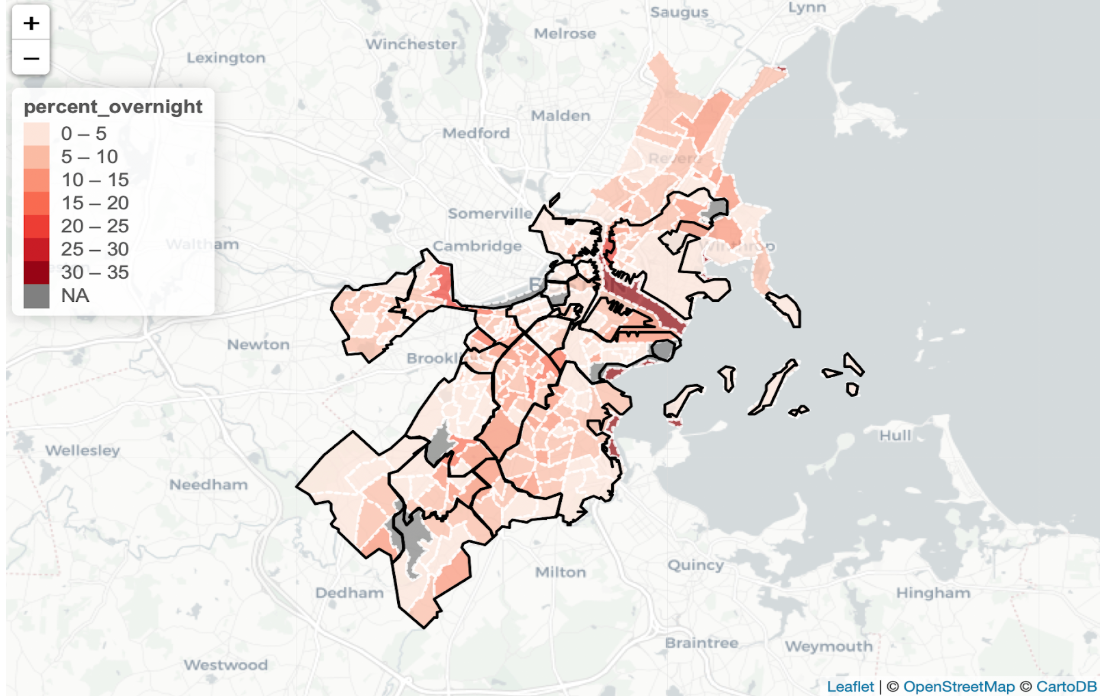
\includegraphics{fig6.png}
\caption{Demand: Percentage maps by tracts of people whose departure
time for home is overnight}
\end{figure}

\begin{figure}
\centering
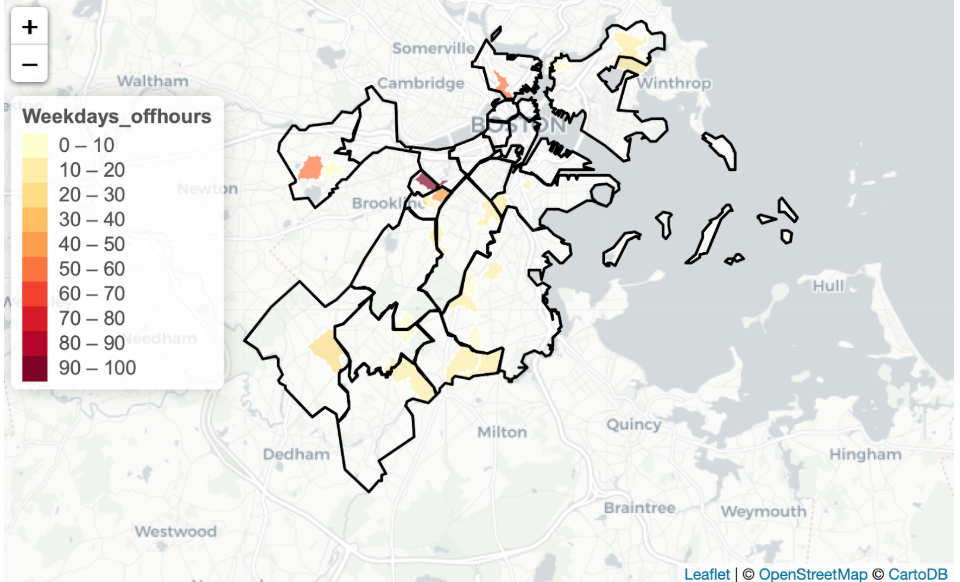
\includegraphics{fig7.png}
\caption{Supply: Number of slots in certain tracts by providers who
operate off hour during weekdays for early ed.}
\end{figure}

\subsection{Data analysis}\label{data-analysis}

We used R (Version 3.4.1; R Core Team, 2017) and the R-packages
\emph{dplyr} (Version 0.8.0.1; Wickham, François, Henry, \& Müller,
2019), \emph{forcats} (Version 0.3.0; Wickham, 2018), \emph{ggformula}
(Version 0.6; D. Kaplan \& Pruim, 2017), \emph{ggplot2} (Version
3.1.0.9000; Wickham, 2016), \emph{lattice} (Version 0.20.35; Sarkar,
2008), \emph{leaflet} (Version 2.0.2; Cheng, Karambelkar, \& Xie, 2018;
Karambelkar \& Schloerke, 2018), \emph{leaflet.extras} (Version 1.0.0;
Karambelkar \& Schloerke, 2018), \emph{mapview} (Version 2.6.3;
Appelhans, Detsch, Reudenbach, \& Woellauer, 2018), \emph{Matrix}
(Version 1.2.10; Bates \& Maechler, 2017), \emph{mosaic} (Version 1.1.0;
Pruim, Kaplan, \& Horton, 2017, 2016), \emph{mosaicData} (Version
0.14.0; Pruim et al., 2016), \emph{papaja} (Version 0.1.0.9842; Aust \&
Barth, 2018), \emph{purrr} (Version 0.3.2; Henry \& Wickham, 2019),
\emph{readr} (Version 1.1.1; Wickham, Hester, \& Francois, 2017),
\emph{sf} (Version 0.7.2; Pebesma, 2018), \emph{stringr} (Version 1.4.0;
Wickham, 2019), \emph{tibble} (Version 2.1.1; Müller \& Wickham, 2019),
\emph{tidycensus} (Version 0.9; Walker, 2019), \emph{tidyr} (Version
0.8.3; Wickham \& Henry, 2019), \emph{tidyverse} (Version 1.2.1;
Wickham, 2017), and \emph{tigris} (Version 0.7; Walker, 2018) for all
our analyses.

\newpage

\section{References}\label{references}

\begin{verbatim}
## [1] "R [Version 3.4.1; @R-base] and the R-packages *dplyr* [Version 0.8.0.1; @R-dplyr], *forcats* [Version 0.3.0; @R-forcats], *ggformula* [Version 0.6; @R-ggformula], *ggplot2* [Version 3.1.0.9000; @R-ggplot2], *lattice* [Version 0.20.35; @R-lattice], *leaflet* [Version 2.0.2; @R-leaflet; @R-leaflet.extras], *leaflet.extras* [Version 1.0.0; @R-leaflet.extras], *mapview* [Version 2.6.3; @R-mapview], *Matrix* [Version 1.2.10; @R-Matrix], *mosaic* [Version 1.1.0; @R-mosaic; @R-mosaicData], *mosaicData* [Version 0.14.0; @R-mosaicData], *papaja* [Version 0.1.0.9842; @R-papaja], *purrr* [Version 0.3.2; @R-purrr], *readr* [Version 1.1.1; @R-readr], *sf* [Version 0.7.2; @R-sf], *stringr* [Version 1.4.0; @R-stringr], *tibble* [Version 2.1.1; @R-tibble], *tidycensus* [Version 0.9; @R-tidycensus], *tidyr* [Version 0.8.3; @R-tidyr], *tidyverse* [Version 1.2.1; @R-tidyverse], and *tigris* [Version 0.7; @R-tigris]"
\end{verbatim}

\begingroup
\setlength{\parindent}{-0.5in} \setlength{\leftskip}{0.5in}

\hypertarget{refs}{}
\hypertarget{ref-R-mapview}{}
Appelhans, T., Detsch, F., Reudenbach, C., \& Woellauer, S. (2018).
\emph{Mapview: Interactive viewing of spatial data in r}. Retrieved from
\url{https://CRAN.R-project.org/package=mapview}

\hypertarget{ref-R-papaja}{}
Aust, F., \& Barth, M. (2018). \emph{papaja: Create APA manuscripts with
R Markdown}. Retrieved from \url{https://github.com/crsh/papaja}

\hypertarget{ref-R-Matrix}{}
Bates, D., \& Maechler, M. (2017). \emph{Matrix: Sparse and dense matrix
classes and methods}. Retrieved from
\url{https://CRAN.R-project.org/package=Matrix}

\hypertarget{ref-R-leaflet}{}
Cheng, J., Karambelkar, B., \& Xie, Y. (2018). \emph{Leaflet: Create
interactive web maps with the javascript 'leaflet' library}. Retrieved
from \url{https://CRAN.R-project.org/package=leaflet}

\hypertarget{ref-R-purrr}{}
Henry, L., \& Wickham, H. (2019). \emph{Purrr: Functional programming
tools}. Retrieved from \url{https://CRAN.R-project.org/package=purrr}

\hypertarget{ref-R-ggformula}{}
Kaplan, D., \& Pruim, R. (2017). \emph{Ggformula: Formula interface to
the grammar of graphics}. Retrieved from
\url{https://CRAN.R-project.org/package=ggformula}

\hypertarget{ref-R-leaflet.extras}{}
Karambelkar, B., \& Schloerke, B. (2018). \emph{Leaflet.extras: Extra
functionality for 'leaflet' package}. Retrieved from
\url{https://CRAN.R-project.org/package=leaflet.extras}

\hypertarget{ref-R-tibble}{}
Müller, K., \& Wickham, H. (2019). \emph{Tibble: Simple data frames}.
Retrieved from \url{https://CRAN.R-project.org/package=tibble}

\hypertarget{ref-R-sf}{}
Pebesma, E. (2018). Simple Features for R: Standardized Support for
Spatial Vector Data. \emph{The R Journal}. Retrieved from
\url{https://journal.r-project.org/archive/2018/RJ-2018-009/index.html}

\hypertarget{ref-R-mosaic}{}
Pruim, R., Kaplan, D. T., \& Horton, N. J. (2017). The mosaic package:
Helping students to 'think with data' using r. \emph{The R Journal},
\emph{9}(1), 77--102. Retrieved from
\url{https://journal.r-project.org/archive/2017/RJ-2017-024/index.html}

\hypertarget{ref-R-mosaicData}{}
Pruim, R., Kaplan, D., \& Horton, N. (2016). \emph{MosaicData: Project
mosaic data sets}. Retrieved from
\url{https://CRAN.R-project.org/package=mosaicData}

\hypertarget{ref-R-base}{}
R Core Team. (2017). \emph{R: A language and environment for statistical
computing}. Vienna, Austria: R Foundation for Statistical Computing.
Retrieved from \url{https://www.R-project.org/}

\hypertarget{ref-R-lattice}{}
Sarkar, D. (2008). \emph{Lattice: Multivariate data visualization with
r}. New York: Springer. Retrieved from
\url{http://lmdvr.r-forge.r-project.org}

\hypertarget{ref-R-tigris}{}
Walker, K. (2018). \emph{Tigris: Load census tiger/line shapefiles}.
Retrieved from \url{https://CRAN.R-project.org/package=tigris}

\hypertarget{ref-R-tidycensus}{}
Walker, K. (2019). \emph{Tidycensus: Load us census boundary and
attribute data as 'tidyverse' and 'sf'-ready data frames}. Retrieved
from \url{https://CRAN.R-project.org/package=tidycensus}

\hypertarget{ref-R-ggplot2}{}
Wickham, H. (2016). \emph{Ggplot2: Elegant graphics for data analysis}.
Springer-Verlag New York. Retrieved from
\url{https://ggplot2.tidyverse.org}

\hypertarget{ref-R-tidyverse}{}
Wickham, H. (2017). \emph{Tidyverse: Easily install and load the
'tidyverse'}. Retrieved from
\url{https://CRAN.R-project.org/package=tidyverse}

\hypertarget{ref-R-forcats}{}
Wickham, H. (2018). \emph{Forcats: Tools for working with categorical
variables (factors)}. Retrieved from
\url{https://CRAN.R-project.org/package=forcats}

\hypertarget{ref-R-stringr}{}
Wickham, H. (2019). \emph{Stringr: Simple, consistent wrappers for
common string operations}. Retrieved from
\url{https://CRAN.R-project.org/package=stringr}

\hypertarget{ref-R-tidyr}{}
Wickham, H., \& Henry, L. (2019). \emph{Tidyr: Easily tidy data with
'spread()' and 'gather()' functions}. Retrieved from
\url{https://CRAN.R-project.org/package=tidyr}

\hypertarget{ref-R-dplyr}{}
Wickham, H., François, R., Henry, L., \& Müller, K. (2019). \emph{Dplyr:
A grammar of data manipulation}. Retrieved from
\url{https://CRAN.R-project.org/package=dplyr}

\hypertarget{ref-R-readr}{}
Wickham, H., Hester, J., \& Francois, R. (2017). \emph{Readr: Read
rectangular text data}. Retrieved from
\url{https://CRAN.R-project.org/package=readr}

\endgroup


\end{document}
